\chapter{6LoCAN design}
\label{cha:design}

The goal of 6LoCAN is to support IPv6 traffic over the CAN-bus with as little overhead as possible.
The payload-data size for classical CAN is eight bytes and for CAN-FD it is 64 bytes.
To satisfy the minimum MTU requirement of 1280 bytes, an efficient fragmentation and reassembly mechanism is required.

Sending IPv6 headers over Classical CAN would at least require six CAN frames, assuming the fragmentation and reassembly header-only takes one byte.
Six frames for only sending the header is not efficient, and therefore, a header compression algorithm is applied.
In the current design, IPHC from 6LoWPAN is used.
In an optimal scenario, the IPv6 and UDP header can be compressed to a size as small as four bytes.

For fragmentation and reassembly, we are using the well known ISO-TP protocol.
ISO-TP can transfer packets with a size of up to 4095 bytes, which is sufficient for the minimal MTU requirements of IPv6.
It also provides a flow-control mechanism for unicast transfers.
ISO-TP does not support multicast transfers, and therefor 6LoCAN uses a slightly modified version that has some simplifications and allows a multicast transfer.
The fragmentation headers designed for 6LoWPAN have a size of four bytes for the first fragment and five bytes for consecutive frames \cite{rfc4944}.
For classical CAN, this is more then the half of the frame payload, which is not efficient enough, and therefore the decision was made not to use it.

CAN uses identifiers to identify frames instead of addresses to address nodes. However, or IPv6 traffic, we need a way to address dedicated nodes.
For this purpose, we introduced an addressing schema that translates node addresses to identifiers.
This schema uses the 29-bit addresses only, and the 11-bit identifiers can still be used for other traffic than 6LoCAN.
The node-addresses defined by the addressing schema have a length of 14 bits and can either be statically assigned or randomly chosen during the initialization of the interface.
Node-addresses need to be unique on the bus. To verify the uniqueness of the node-address, we introduced a Link-Layer duplicate address detection.

This work also defines a translator from the 6LoCAN network to an Ethernet-based network.
We named this translator mechanism a 6LoCAN border translator.
The translator makes it possible to connect 6LoCAN nodes with Ethernet nodes on the same Link-Local domain.
The translator can then be connected to another node, an Ethernet-Switch, Router, or whatever device using Ethernet.
The translator is stateless and has a fixed address. Because of the fixed address, it does not need to be advertised among nodes,
but we can only have a single translator within a 6LoCAN network. 

\section{Addressing Schema}
\label{sec:addressing_schema}

\begin{figure}[htp]
	\begin{center}
	\begin{tikzpicture}[scale=0.35,  every node/.style={scale=0.35},
		region/.style={
			rectangle, 
			minimum height=1.5cm,
			font=\huge}]

		\node (mcast) [region, minimum width=1cm] {M};
		\node (dest) [region, right of=mcast,xshift=6.5cm, minimum width=14cm] {DEST};
		\node (src) [region, right of=dest,xshift=13cm, minimum width=14cm] {SRC};

		\draw (mcast.north west) -- (src.north east);
		\draw (mcast.south west) -- (src.south east);
		\draw (mcast.south west) -- ++(0,2.5cm);
		\draw (mcast.south east) -- ++(0,2.5cm);
		\draw (dest.south east) -- ++(0,2.5cm);
		\draw (src.south east) -- ++(0,2.5cm);
		\draw[<->] ($(mcast.north west) + (0,0.5cm)$) -- ($(mcast.north east) + (0,0.5cm)$) node[midway, above] {\huge 1};
		\draw[<->] ($(mcast.north east) + (0,0.5cm)$) -- ($(dest.north east) + (0,0.5cm)$) node[midway, above] {\huge 14};
		\draw[<->] ($(dest.north east) + (0,0.5cm)$) -- ($(src.north east) + (0,0.5cm)$) node[midway, above] {\huge 14};
	\end{tikzpicture}
	\caption{Address to Identifier Mapping}
	\label{fig:des_addr_to_id}
	\end{center}
\end{figure}

6LoCAN uses 14-bit node addresses to identify nodes on the bus.
A node address has to be unique on the bus to avoid collisions.
The Link-Layer duplicate address detection, defined in \autoref{sec:lldad}, prevents node address collisions.
The addressing schema describes how to map the 14-bit source and destination node-address to a 29-bit CAN identifier, as shown in \autoref{fig:des_addr_to_id}.
The resulting CAN identifier is a combination of the source address, destination address, and a multicast bit.
Because of the fact that a node address must be unique on the bus, the combination of the source and destination address always results in a unique identifier.
This property is essential because collisions on the bus can only be resolved during the arbitration phase.
If two nodes would send frames with the same identifiers, a collision in the data-phase could happen that cannot be resolved.
Mapping only the destination address int the identifier would extend the address-space but leads to collision when two nodes try to send data to the same receiver.
Mapping only the source address to the identifier would not lead to collisions, but the nodes would need to inspect every packet, and the destination address would need to be included in every frame payload.
With having the destination-node address as part of the identifier, the 6LoCAN node can use masked CAN filters to only receive frames dedicated to the node.
This method reduces the number of interrupts for receiving and parsing frames.
A dedicated multicast-bit marks frames as multicast frames.
A node can use a masked CAN filter to receive multicast traffic from the attached multicast groups only.

\begin{table}
	\centering
	\caption{6LoCAN address layout}
	\begin{tabular}{|c|l|} \hline
	Address         & Description         \\ \hline \hline
	0x3DFE - 0x3FFF & Reserved            \\ \hline
	0x3DFE          & LLDAD               \\ \hline
        0x3DF1 - 0x3DFD & Reserved            \\ \hline
        0x3DF0          & Ethernet Translator \\ \hline
        0x0100 - 0x3DEF & Node addresses      \\ \hline
        0x0000 - 0x00FF & Reserved            \\ \hline
	\end{tabular}
        \label{tab:address_layout}
\end{table}

\autoref{tab:address_layout} describes the address layout.
Nodes can use any address from 0x0100 to 0x3DEF.
Other addresses are either reserved or used for a particular purpose.

The conclusion of the addressing schema leads to the following properties:
\begin{itemize}
        \item 14-bit address-space on the bus.
        \item The identifier uniquely identifies traffic from one node to another.
        \item The combination of source and destination address prevents collisions outside the arbitration-field.
        \item CAN filters that only pass relevant frames can easily be applied to the identifiers.
\end{itemize}

\newpage

\subsection{Unicast Address}
\label{sec:unicast_addr}

\begin{figure}[htp]
	\begin{center}
	\begin{tikzpicture}[scale=0.35,  every node/.style={scale=0.35},
		region/.style={
			rectangle, 
			minimum height=1.5cm,
			font=\huge}]

		\node (mcast) [region, minimum width=1cm] {0};
		\node (dest) [region, right of=mcast,xshift=6.5cm, minimum width=14cm] {DEST Node-Address};
		\node (src) [region, right of=dest,xshift=13cm, minimum width=14cm] {SRC Node-Address};

		\draw (mcast.north west) -- (src.north east);
		\draw (mcast.south west) -- (src.south east);
		\draw (mcast.south west) -- ++(0,2.5cm);
		\draw (mcast.south east) -- ++(0,2.5cm);
		\draw (dest.south east) -- ++(0,2.5cm);
		\draw (src.south east) -- ++(0,2.5cm);
		\draw[<->] ($(mcast.north west) + (0,0.5cm)$) -- ($(mcast.north east) + (0,0.5cm)$) node[midway, above] {\huge 1};
		\draw[<->] ($(mcast.north east) + (0,0.5cm)$) -- ($(dest.north east) + (0,0.5cm)$) node[midway, above] {\huge 14};
		\draw[<->] ($(dest.north east) + (0,0.5cm)$) -- ($(src.north east) + (0,0.5cm)$) node[midway, above] {\huge 14};
	\end{tikzpicture}
	\caption{Unicast Node-Address to Identifier Mapping}
	\label{fig:des_unicast_addr_to_id}
	\end{center}
\end{figure}

\autoref{fig:des_unicast_addr_to_id} depicts the mapping from source node-address and destination node-address to the CAN identifier for unicast traffic.
The uppermost bit, the multicast bit, is set to zero.
The destination node-address is located in the upper 14 bits, and the source node-address is located in the lower 14 bits.


\subsection{Multicast Address}
\label{sec:multicast_addr}

\begin{figure}[htp]
	\begin{center}
	\begin{tikzpicture}[scale=0.35,  every node/.style={scale=0.35},
		region/.style={
			rectangle, 
			minimum height=1.5cm,
			font=\huge}]

		\node (mcast) [region, minimum width=1cm] {1};
		\node (dest) [region, right of=mcast,xshift=6.5cm, minimum width=14cm] {Multicast-Group};
		\node (src) [region, right of=dest,xshift=13cm, minimum width=14cm] {SRC Node-Address};

		\draw (mcast.north west) -- (src.north east);
		\draw (mcast.south west) -- (src.south east);
		\draw (mcast.south west) -- ++(0,2.5cm);
		\draw (mcast.south east) -- ++(0,2.5cm);
		\draw (dest.south east) -- ++(0,2.5cm);
		\draw (src.south east) -- ++(0,2.5cm);
		\draw[<->] ($(mcast.north west) + (0,0.5cm)$) -- ($(mcast.north east) + (0,0.5cm)$) node[midway, above] {\huge 1};
		\draw[<->] ($(mcast.north east) + (0,0.5cm)$) -- ($(dest.north east) + (0,0.5cm)$) node[midway, above] {\huge 14};
		\draw[<->] ($(dest.north east) + (0,0.5cm)$) -- ($(src.north east) + (0,0.5cm)$) node[midway, above] {\huge 14};
	\end{tikzpicture}
	\caption{Multicast-Group to Identifier Mapping}
	\label{fig:des_multicast_to_id}
	\end{center}
\end{figure}

\autoref{fig:des_multicast_to_id} depicts the mapping from source node-address and the multicast group to the CAN identifier for multicast traffic.
The uppermost bit, the multicast bit, is set to one.
The desired multicast group is located in the upper 14 bits, and the source node-address is located in the lower 14 bits.
The multicast group corresponds to the lower 14 bits of the IPv6 multicast address.
As shown in \autoref{sec:ipv6} \autoref{fig:ipv6_multicast_addr}, the Group-ID is located at the lower 112 bits of the IP address.
Using the lower 14 bits is very efficient because all well-known multicast groups fit in that range.
The node can also receive messages with a multicast Group-ID larger than 14 bits,
but these messages may be ambiguous and need to be filtered afterward by the IPv6 address.

\subsection{Address Generation}
\label{sec:address_generation}

Every node is addressed by a 14-bit address as described in \autoref{sec:addressing_schema}.
A node can either have a statically assigned address, or it can pick a random address whenever it connects to the bus or restarts the interface.
In the case of a random address assignment, multiple nodes might attempt to claim the same address at the same time.
Two nodes with the same address would be a violation of the requirement that every node must have a unique address on the bus.
To prevent this situation, \autoref{sec:lldad} describes a mechanism to detect address duplications on the bus.
A node that tries to claim an address already in use can then choose another address and rerun the detection for duplicate addresses.

Random address assignment allows nodes to join the network without any prior knowledge of the other nodes and without being provisioned first.
It is especially useful for nodes that do not have an interface to enter an address or lack of none volatile memory.
The drawback is that the address of a node may change their address whenever it reenters the network.

\subsection{Link-Layer Duplicate Address Detection}
\label{sec:lldad}

To evaluate the need of the Link-Layer duplicate address detection lets first calculate the probability that two devices choose the same address,
when they use an independent random number to assign their address.
The address space a node can take its address from is 0x0100 to 0x3DEF (15599).
Let us assume that we have 100 nodes on the bus.
Depending on the transceivers used and wiring, this is a realistic electrical limit.

Let $N$ be the number of possible addresses, $n$ the number of nodes, and $P$ the probability for a collision. 
The number of possible permutations of addresses and nodes is $N^n = 15599^{100}$.\\
The number of permutations without a collision is \\ $N \cdot (N-1) \cdot ... \cdot (N - (n - 1))$.\\
Using the Laplace formula gives \autoref{eq:prop_col}.

\begin{equation}
	\begin{split}
		P = 1 - \frac{N \cdot (N-1) \cdot ... \cdot (N - (n - 1))}{N^n} \\
		P = 1 - \frac{\displaystyle\prod_{i=1}^{n} N - (i - 1)}{N^n} = 1 -\frac{n! \cdot \binom{N}{n}} {N^n}
	\end{split}
	\label{eq:prop_col}
	\end{equation}
	
	\begin{equation}
		P = 1 - \frac{100! \cdot \binom{15599}{100}}{15599^{100}} \approx 0.2724
	\label{eq:prop_col_res}
	\end{equation}

\autoref{eq:prop_col_res} is the result of our example with 100 nodes.

The probability of having a collision is therefor 27.24\%.
For most applications, this number unacceptable, and a mechanism to prevent collisions needs to be applied.

For this reason, we introduced the Link-Layer duplicate address detection (LLDAD).
LLDAD works on the Link-Layer only and utilizes a special CAN frame type, the Remote Transmission Request (RTR).

\begin{figure}[htp]
	\begin{center}
	\begin{tikzpicture}[scale=0.35,  every node/.style={scale=0.35},
		region/.style={
			rectangle,
			draw=black,
			minimum height=1.5cm,
			font=\huge}]

		\node (mcast) [region, minimum width=1cm] {0};
		\node (dest) [region, right of=mcast,xshift=6.5cm, minimum width=14cm] {Tentative Address};
		\node (src) [region, right of=dest,xshift=13cm, minimum width=14cm] {entropy};

		\draw (mcast.north west) -- (src.north east);
		\draw (mcast.south west) -- (src.south east);
		\draw (mcast.south west) -- ++(0,2.5cm);
		\draw (mcast.south east) -- ++(0,2.5cm);
		\draw (dest.south east) -- ++(0,2.5cm);
		\draw (src.south east) -- ++(0,2.5cm);
		\draw[<->] ($(mcast.north west) + (0,0.5cm)$) -- ($(mcast.north east) + (0,0.5cm)$) node[midway, above] {\large 1};
		\draw[<->] ($(mcast.north east) + (0,0.5cm)$) -- ($(dest.north east) + (0,0.5cm)$) node[midway, above] {\large 14};
		\draw[<->] ($(dest.north east) + (0,0.5cm)$) -- ($(src.north east) + (0,0.5cm)$) node[midway, above] {\large 14};
	\end{tikzpicture}
	\caption{Link-Layer Duplicate Address Detection Request Frame}
	\label{fig:des_lldad_req}
	\end{center}
\end{figure}

The collision detection begins with sending an LLDAD-request.
The LLDAD-request is an RTR frame with no data.
The 29-bit identifier has the same address-layout as a unicast 6LoCAN frame, but the source address is filled with entropy,
and the destination address is filled with the tentative address as shown in  \autoref{fig:des_lldad_req}.
The entropy prevents collisions in case another node tries to acquire the same address at the same time.
The probability of not having a collision with 100 nodes, performing LLDAD at the same time, is calculated in \autoref{eq:prop_col_dad}.
The equation uses a slightly modified formula from \autoref{eq:prop_col} with an address range extended by the 14-bit entropy.

\begin{equation}
	P = \frac{100! \cdot \binom{15599 \cdot 2^{14}}{100}}{(15599 \cdot 2^{14})^{100}} \approx 0.99998
\label{eq:prop_col_dad}
\end{equation}

\begin{figure}[htp]
	\begin{center}
	\begin{tikzpicture}[scale=0.35,  every node/.style={scale=0.35},
		region/.style={
			rectangle,
			draw=black,
			minimum height=1.5cm,
			font=\huge}]

		\node (mcast) [region, minimum width=1cm] {0};
		\node (dest) [region, right of=mcast,xshift=6.5cm, minimum width=14cm] {0x3DFE};
		\node (src) [region, right of=dest,xshift=13cm, minimum width=14cm] {Tentative Address};

		\draw (mcast.north west) -- (src.north east);
		\draw (mcast.south west) -- (src.south east);
		\draw (mcast.south west) -- ++(0,2.5cm);
		\draw (mcast.south east) -- ++(0,2.5cm);
		\draw (dest.south east) -- ++(0,2.5cm);
		\draw (src.south east) -- ++(0,2.5cm);
		\draw[<->] ($(mcast.north west) + (0,0.5cm)$) -- ($(mcast.north east) + (0,0.5cm)$) node[midway, above] {\large 1};
		\draw[<->] ($(mcast.north east) + (0,0.5cm)$) -- ($(dest.north east) + (0,0.5cm)$) node[midway, above] {\large 14};
		\draw[<->] ($(dest.north east) + (0,0.5cm)$) -- ($(src.north east) + (0,0.5cm)$) node[midway, above] {\large 14};
	\end{tikzpicture}
	\caption{Link-Layer Duplicate Address Detection Response Frame}
	\label{fig:des_lldad_resp}
	\end{center}
\end{figure}

After the LLDAD-request is sent, the node waits at least 100ms for an LLDAD response frame.
The response-frame is not an RTR frame and does not contain data.
The identifier of the response is shown in \autoref{fig:des_lldad_resp}.
The destination-address is the LLDAD response address 0x3DFE, and the source address is the address of the node that already owns the address,
which is the same address as the tentative address.
If there is no LLDAD-response frame with the tentative address as the source address on the bus,
the tentative address is considered to be unique and becomes the address of the node.
If the node receives an LLDAD-response, the LLDAD is failed, and in case the address was randomly chosen, it can retry with another random address.
If the address was statically assigned, the node is not allowed to use the address and, therefore, cannot bring up the interface.

\begin{figure}[htp]
	\begin{center}
	\begin{tikzpicture}[scale=0.6, node distance=2cm, every node/.append style={scale=0.6}]
		\node (start) [startstop] {Interface Up};
		\node (ll_ten) [process, below = of start] {Chose Tentative Link-Local Address (static address or random)};
		\node (lldad_req) [io, below = of ll_ten] {Send LLDAD-Request};
		\node (lldad_resp) [io, below = of lldad_req] {Wait for LLDAD-Response or 100ms Timeout};
		\node (lldad) [decision, below = of lldad_resp] {LLDAD-Response received?};
		\node (rand) [decision, right of=lldad, xshift=7cm] {Random address?};
		\node (lldad_fail) [startstop, below = of rand] {LLDAD failed};
		\node (success) [startstop, below = of lldad] {Use Tentative Address as Node Address};

		\draw [arrow] (start) -- (ll_ten);
		\draw [arrow] (ll_ten) -- (lldad_req);
		\draw [arrow] (lldad_req) -- (lldad_resp);
		\draw [arrow] (lldad_resp) -- (lldad);
		\draw [arrow] (lldad) -- node [anchor=south] {yes (LLDAD failed)} (rand);
		\draw [arrow] (lldad) -- node [anchor=east] {no (LLDAD succeeded)} (success);
		\draw [arrow] (rand) |- node [anchor=south] {yes} (ll_ten);
		\draw [arrow] (rand) -- node [anchor=east] {no} (lldad_fail);
	\end{tikzpicture}
	\end{center}
	\caption{Link-Layer Duplicate Address Detection}
	\label{fig:des_lldad}
\end{figure}

\autoref{fig:des_lldad} depicts the procedure of the LLDAD.

\section{Stateless Address Autoconfiguration}
\label{sec:impl_slaac}

The process of creating an IPv6 address is defined in \autoref{sec:ipv6_slaac}.
However, forming the interface identifier depends on the underlying Link-Layer.
The process of creating an interface identifier does not strictly follow the rules of RFC4291 \cite{rfc4291} Appendix A.
Instead of taking the 14-bit node address and zero fill it to the left, we use the method of creating an identifier from a 48-bit identifier.
The reason for this is that this method was also chosen for 6LoWPAN (RFC4944 \cite{rfc4944}) and the header compression
is most efficient when the interface identifier if formed in that way.

For example, a node with the node-address of 0x1234 would create the interface identifier ::ff:fe00:1234/64.

Since the node address is only guaranteed to be unique on the bus-segment, the IPv6 Duplicate Address detection,
as described in \autoref{sec:ipv6_slaac}, needs to be performed.
If the DAD failed, the node can either pick a new node-address or form an interface identifier that is not related to the node-address.
The latter would result in an inefficient header compression and should, therefore, be avoided.

\section{ISO-TP for 6LoCAN}
\label{sec:iso_tp_6LoCAN}

IPv6 defines that the minimal MTU is 1280 bytes, but a CAN frame has a payload length of eight bytes for classical CAN and 64 bytes for CAN-FD.
To satisfy the minimal MTU requirement, 6LoCAN uses a slightly modified version of ISO-TP.
Some features like the address extension are not useful and, therefore, not used and not supported.
The maximum packet size is limited to 4095 bytes, to limit the PCI of the first frame to two bytes.
TSO-TP does only support unicast data transfer, but for IPv6, it is necessary to have multicast traffic too.
Hence, we defined a way to have multicast transmissions, but without flow control.

\subsection{Multicast}
\label{sec:multicast_iso_tp}

For multicast packets, we cannot have flow control, because there is more than one node receiving the packet and therefore,
more than one node that would answer with a flow control frame.
The sender cannot handle flow control for more than one receiving node because he does not know who and how many receivers there are.

\begin{figure}[htp]
\begin{center}
	\begin{tikzpicture}[scale=0.7]
		%Sender
		\node (s_ff) at (0,10)  {};
		\node (s_cf1) at (0,7) {};
		\node (s_cf2) at (0,5) {};
		\node (s_cf3) at (0,3) {};
		
		%Receiver
		\node (r_ff) at (12,9)  {};
		\node (r_cf1) at (12,6) {};
		\node (r_cf2) at (12,4) {};
		\node (r_cf3) at (12,2) {};


		%connections
		\draw[thick, ->] (s_ff) -- node[midway, fill=white] {First Frame} (r_ff);
		\draw[thick,->] (s_cf1) -- node[midway, fill=white] {Consecutive Frame} (r_cf1);
		\draw[thick,->] (s_cf2) -- node[midway, fill=white] {Consecutive Frame} (r_cf2);
		\draw[thick,->] (s_cf3) -- node[midway, fill=white] {Consecutive Frame} (r_cf3);
		
		%FF - CF time
		\draw (r_ff) -- ++(2,0);
		\draw (s_cf1) -- ++(14,0);
		\draw[<->] ($(r_ff) + (1,0)$) -- ($(s_cf1) + (13,0)$) node[midway,right]{\small 1ms};

		%stmin
		\draw (r_cf2) -- ++(2,0);
		\draw (s_cf3) -- ++(14,0);
		\draw[<->] ($(r_cf2) + (1,0)$) -- ($(s_cf3) + (13,0)$) node[midway,right]{\small $ST_{min}$};
		
		%Flow
		\draw[very thick, ->] (0,10.5) --  (0,0);
		\node at (0,11) {Sender};
		\draw[very thick, ->] (12,10.5) -- (12,0);
		\node at (12,11) {Receiver};
		
	\end{tikzpicture}
	\caption{Example Multicast Sequence}
	\label{fig:des_iso_tp_mcast}
\end{center}
\end{figure}

\autoref{fig:des_iso_tp_mcast} shows the sequence of a multicast transfer.
6LoCAN defines that there has to be a pause between the First Frame and the first Consecutive Frame of at least 1ms.
This pause allows all receiving nodes to set-up the CAN filter and allocate memory for the reception of the frame.
The $ST_{min}$ has to be chosen such that the slowest node on the bus can handle the reception.
Multicast traffic is slower and maybe more unreliable than unicast transfers.
For packets that fit in a Single Frame packet, multicast works the same way as unicast does.

\subsection{Ethernet Border Translator}
\label{sec:eth_border_translator}

\begin{figure}
    \begin{center}
	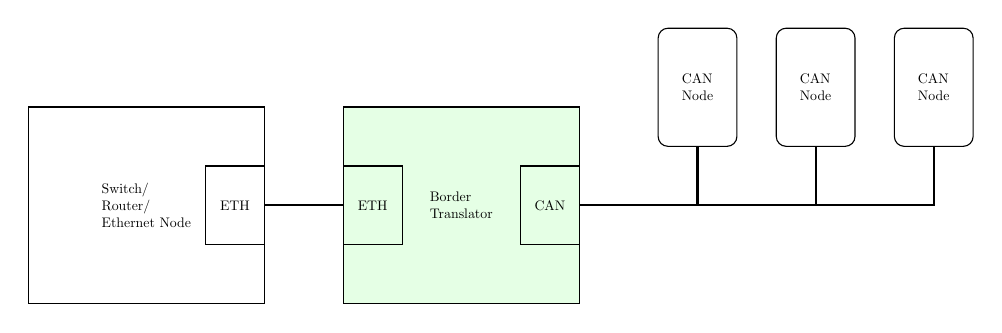
\begin{tikzpicture}[scale=0.5,  every node/.style={scale=0.5},
		rect/.style={
			draw,
			minimum height=5cm,
			minimum width=6cm,
			align=left},
			iface/.style={
			draw,
			minimum height=2cm,
			minimum width=1.5cm},
			can/.style={
			draw,
			align=left,
			minimum height=3cm,
			minimum width=2cm,
			rounded corners=0.125cm}]

		\node (switch) [rect] {Switch/ \\Router/ \\Ethernet Node};
		\node (switchEth) [iface, right of = switch, xshift=1.25cm] {ETH};

		\node (bt) [rect, fill=green!10, right of = switch, xshift=7cm] {Border \\Translator};
		\node (bteth) [iface, left of = bt, xshift=-1.25cm] {ETH};
		\node (btcan) [iface, right of = bt, xshift=1.25cm] {CAN};

		\node (can1) [can, right of = bt, xshift=5cm, yshift=3cm] {CAN \\Node};
		\node (can2) [can, right of = can1, xshift=2cm] {CAN \\Node};
		\node (can3) [can, right of = can2, xshift=2cm] {CAN \\Node};

		\draw [thick] (switchEth) -- (bteth);
		\draw [thick] (btcan) -| (can1);
		\draw [thick] (btcan) -| (can2);
		\draw [thick] (btcan) -| (can3);
	\end{tikzpicture}
	\caption{Ethernet Border Translator Schematic}
	\label{fig:bordertrans}
	\end{center}
\end{figure}

The Ethernet Border Translator is a concept for connecting a 6LoCAN bus segment to an Ethernet network.
It is neither a router nor a switch.
It only translates the packets from one Link-Layer to another, which means that the nodes stay in the same Link-Local domain.
The advantage of this concept is that the translator is fully stateless and does not need any configuration and knowledge of the network.
It allows us to use small devices with very little memory to be used as Border Translators.
In case the 6LoCAN network segment needs a router, the Border Translator can be used to connect the 6LoCAN network to an ordinary Ethernet router.
The Ethernet Border Translator can also be used to connect multiple 6LoCAN bus segments, using a standard Ethernet Switch.
With the Ethernet Border Translator, we can use already existing Ethernet equipment for routing 6LoCAN traffic in the network.
The advantage of keeping the devices in the same Link-Local domain is that multicast discovery protocols still works.

The translator has a fixed CAN node address (0x3DF0).
With having a fixed address for the translator, the other nodes do not need a mechanism for discovering translators.
6LoCAN nodes do not need to know if a destination node the want to reach is in the same network, or connected via a translator.
The sending node only needs to perform a neighborhood discovery as described in \autoref{sec:ipv6_ndp}.
The border translator then forwards the neighbor solicitation message, and if the node is behind the translator,
the answer will be forwarded by the translator.
Since the address of the translator is well known, a node automatically knows that the packet is from outside the CAN bus segment,
if the source node-address is the translator address.
Packets forwarded from Ethernet to 6LoCAN carry the original 48 bit Ethernet MAC address directly after the ISO-TP First Frame header.
Since the First Frame header has a size of two bytes, the inlined address always fits in the remaining frame data.
A node receiving a packet from the border translator now replaces the node-address with the in-lined MAC address and saves it to the neighborhood cache.
The node can now decide from the size of the address, stored in the neighborhood cache,
if the packets need to be sent to the translator or to a node within the same bus-segment.
Packets originating from a 6LoCAN node with a destination behind the translator are sent to the node-address of the translator
and carry the destination Ethernet MAC-address inline.
The border translator reassembles the packet, uncompresses the IPv6 header, and forwards the packet to the destination MAC-address.
The source MAC-address is the 14-bit 6loCAN node-address extended by a 34-bit prefix.
For packets from Ethernet to 6LoCAN, the translator compresses the IPv6 header and performs an ISO-TP transmission to the destination node.
The destination node-address is taken from the last 14 bits of the destination MAC-address.

For neighborhood discovery packets, originating from the 6LoCAN network, with a Link-Layer address option (see \autoref{sec:ipv6_ndp}),
the translator has to inspect the packet and extend the address in the option to match the extended Ethernet MAC-address.

\begin{figure}[htp]
	\begin{center}
	\begin{tikzpicture}[scale=0.4,  every node/.style={scale=0.4},
		region/.style={
			rectangle,
			draw,
			align=center,
			font=\Large,
			minimum height=2cm}]

		\node (mcast) [region, minimum width=1cm] {0};
		\node (dest) [region, right of=mcast,xshift=1.5cm, minimum width=4cm] { DEST (0x3DF0)};
		\node (src) [region, right of=dest,xshift=3cm, minimum width=4cm] {SRC (0x123)};
		\node (dstmacil) [region, right of=src,xshift=4cm, minimum width=6cm] {Inlined DEST MAC};

		\node (dstmac) [region, right of=dstmacil, xshift=9cm, minimum width=7cm] {DEST MAC};
		\node (srcmac) [region, right of=dstmac, xshift=6cm, minimum width=7cm] {SRC MAC \\ (DE:AD:BE:EF:01:23)};

		\draw[thick, ->] (dstmacil.east) -- (dstmac.west) coordinate[midway](border);
		\draw[dashed, black!50] ($(border) + (0,-3cm)$) -- ($(border) + (0,4.5cm)$);
		\node at ($(border) + (-2cm,3.5cm)$) {\Huge 6LoCAN};
		\node at ($(border) + (2cm,3.5cm)$) {\Huge Ethernet};
		\draw[->] (dstmacil.south) .. controls ++(5cm,-1.5cm) .. (dstmac.south);
		\draw[->] (src.north) .. controls ++(9cm,1.5cm) .. (srcmac.north) node [align=center, very near start, above, yshift=0.25cm] {\Large Extend with Prefix \\ \Large(DE:AD:BE:EF)};
	\end{tikzpicture}
	\caption{6LoCAN to Ethernet Address Translation}
	\label{fig:bordertrans_6lo_eth}
	\end{center}
\end{figure}
\begin{figure}[htp]
	\begin{center}
	\begin{tikzpicture}[scale=0.4,  every node/.style={scale=0.4},
		region/.style={
			rectangle,
			draw,
			font=\Large,
			align=center,
			minimum height=2cm}]

		\node (dstmac) [region,, minimum width=7cm] {DST MAC \\ (DE:AD:BE:EF:01:23)};
		\node (srcmac) [region, right of=dstmac, xshift=6cm, minimum width=7cm] {SRC MAC};

		\node (mcast) [region,right of=srcmac, xshift=6cm, minimum width=1cm] {0};
		\node (dest) [region, right of=mcast,xshift=1.5cm, minimum width=4cm] {DEST (0x123)};
		\node (src) [region, right of=dest,xshift=3cm, minimum width=4cm] {SRC (0x3DF0)};
		\node (dstmacil) [region, right of=src,xshift=4cm, minimum width=6cm] {Inlined SRC MAC};

		\draw[thick, ->] (srcmac.east) -- (mcast.west) coordinate[midway](border);
		\draw[dashed, black!50] ($(border) + (0,-3cm)$) -- ($(border) + (0,4.5cm)$);
		\node at ($(border) + (-2cm,3.5cm)$) {\Huge Ethernet};
		\node at ($(border) + (2cm,3.5cm)$) {\Huge 6LoCAN};
		\draw[->] (srcmac.south) .. controls ++(10cm,-1.5cm) .. (dstmacil.south);
		\draw[->] (dstmac.north) .. controls ++(9cm,1.5cm) .. (dest.north) node [align=center, very near start, above, yshift=0.25cm]{\Large Take the last 14 bits};
	\end{tikzpicture}
	\caption{Ethernet to 6LoCAN Address Translation}
	\label{fig:bordertrans_eth_6lo}
	\end{center}
\end{figure}

\autoref{fig:bordertrans_6lo_eth} shows how the 6LoCAN node address is extended to an Ethernet MAC-address and 
\autoref{fig:bordertrans_eth_6lo} shows how the Ethernet MAC-address address is extended to a 6LoCAN node address.
